\tableofcontents

\newpage



\section{Описание метода}
Разобьем отрезок интегрирования $[a, b]$ на четное число $n$ равных частей с шагом $h$. На
каждом отрезке $[x_0, x_2]$, $[x_2, x_4]$, …, $[x_{i-1}, x_{i+1}]$, … , $[x_{n-2}, x_n]$
$s_i$ = $\frac{h}{3}$$(y_{i-1} + 4y_i + y_{i+1})$, а $S$ = $\sum\limits_{i=1}^{n} s_i$. \\
Увеличиваем n в 2 раза и повторяем до тех пор, пока разница в вычислениях между итерациями не будет $\leq$ $\epsilon$


\section{Блок-схема численного метода}
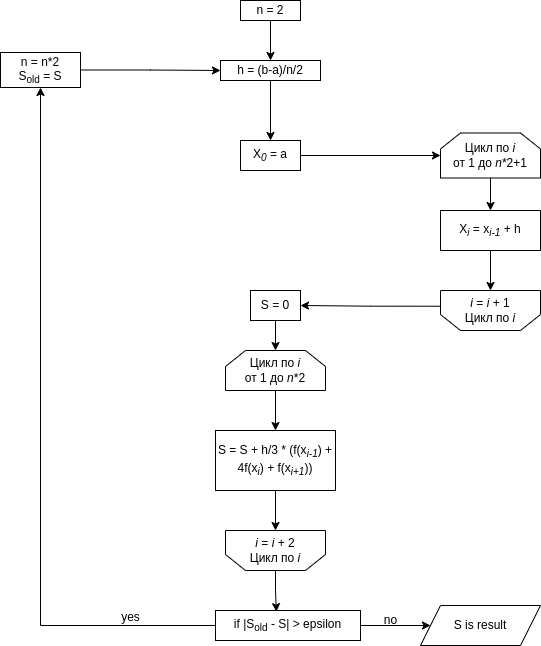
\includegraphics[scale=0.3]{img/integrity}

\section{Listing реализованного численного метода}
\tiny
\begin{verbatim}
    public double integrate(SimpleFunction f, double a, double b, double epsilon) {
        int n=2;
        double h = IntegrationBySimpsonCalculator.calcutaleH(a, b, n);
        double[] segments = IntegrationBySimpsonCalculator.sectioning(a, n, h);
        double resOld = IntegrationBySimpsonCalculator.integration(f, segments, h);
        n*=2;
        h = IntegrationBySimpsonCalculator.calcutaleH(a, b, n);
        segments = IntegrationBySimpsonCalculator.sectioning(a, n, h);
        double resNew = IntegrationBySimpsonCalculator.integration(f, segments, h);
        while (Math.abs(resNew - resOld) > epsilon) {
            resOld = resNew;
            n*=2;
            h = IntegrationBySimpsonCalculator.calcutaleH(a, b, n);
            segments = IntegrationBySimpsonCalculator.sectioning(a, n, h);
            resNew = IntegrationBySimpsonCalculator.integration(f, segments, h);
        }
        return resNew;
    }

    static double integration(SimpleFunction f, double[] X, double h){
        double S = 0;
        for (int i=1; i<X.length -1; i++) {
            S += integratePart(f, X[i-1], X[i], X[i+1], h);
            i++;
        }
        return S;
    }

    static double calcutaleH(double a, double b, int n) {
        return (b-a)/n/2;
    }

    static double[] sectioning(double a, int n, double h) {
        double x=a;
        double[] X = new double[n*2+1];
        for (int i=0; i<X.length; i++) {
            X[i] = x;
            x+=h;
        }
        return X;
    }

    private static double integratePart(SimpleFunction f, double z, double o, double v, double h) {
        return h/3*(f.apply(z) + f.apply(o)*4 + f.apply(v));
    }

\end{verbatim}
\normalsize

\section{Examples}
\begin{verbatim}
Choose the function that you want to integrate:
1. f(x) = x²
2. f(x) = sin(x)/x
3. f(x) = 1000x - 7
4. f(x) = sqrt(x)

2

In this function, the discontinuity of the first kind at x=0 is eliminated by the
definition of the function at this point f(0) = 0.

Enter the left boundary of the integration: -5
Enter the right boundary of the integration: 3
Set the accuracy of calculations: 0.0001
Result of integration: 3.398502392735804


Choose the function that you want to integrate:
1. f(x) = x²
2. f(x) = sin(x)/x
3. f(x) = 1000x - 7
4. f(x) = sqrt(x)

3

Enter the left boundary of the integration: -1
Enter the right boundary of the integration: 1
Set the accuracy of calculations: 0.00001
Result of integration: -14.0

\end{verbatim}


\section{Вывод}
Точность метода Симпсона выше точности метода прямоугольников и трапеций для заданного n, так
что его использование предпочтительнее в общем случае. Однако, при больших n зачастую накапливается
погрешность вычислений в результате многочисленных арифметических действия, что может отдалить приближенное значение от точного.
Поэтому, если заранее аналитически известно, что график функции достаточно "прямой" - лучше воспользоваться
другими методами, и получить точное решение при меньших n.
